\documentclass[aspectratio=169]{beamer}

% -------- theme + packages --------
\usetheme{default}
\usecolortheme{dove}
\useinnertheme{rectangles}
\setbeamertemplate{navigation symbols}{}
\setbeamertemplate{footline}[frame number]
\setbeamercolor{frametitle}{fg=black}
\setbeamerfont{frametitle}{series=\bfseries}

\usepackage{amsmath,amssymb}
\usepackage{graphicx}
\usepackage{tikz}
\usetikzlibrary{positioning, arrows.meta, shapes}
\usepackage{xcolor}
\usepackage{booktabs}
\usepackage{array}
\usepackage{makecell}
\usepackage{tcolorbox}

\definecolor{harmred}{RGB}{198,40,40}
\definecolor{safegreen}{RGB}{46,125,50}
\definecolor{neutralblue}{RGB}{21,101,192}
\definecolor{warnorange}{RGB}{245,127,23}
\definecolor{mutedgray}{RGB}{117,117,117}
\definecolor{highlightyellow}{RGB}{255,248,225}

% -------- title --------
\title{\textbf{Dynamically Identifying a Safe/Harmful Subset of Experts in Mixture-of-Experts (MoE) Models}}
\author{}
\date{}

\begin{document}

% ================================================================
% Title
% ================================================================
\begin{frame}
  \titlepage
\end{frame}

% ================================================================
% Slide 1: MoE intro  — keep simple
% ================================================================
\begin{frame}{MoE LLMs: many small experts, pick a few per word}
\vspace{-0.2em}
  \begin{columns}[T]
    \begin{column}{0.55\textwidth}
      \begin{itemize}
        \setlength\itemsep{0.45em}
        \item Each transformer layer has \textbf{many small FFN experts}
          (often 64 or 512).
        \item A \textbf{router} looks at the current word and selects only a
          \textbf{few experts} (e.g.\ top-8) to contribute.
        \item The final output is the weighted sum of the selected experts.
      \end{itemize}
    \end{column}
    \begin{column}{0.42\textwidth}
      \centering
      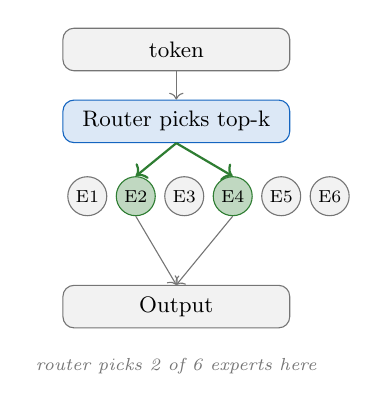
\begin{tikzpicture}[node distance=0.15cm, scale=0.9, transform shape]
        \node[rectangle, rounded corners, draw=mutedgray, fill=gray!10,
              minimum width=3.2cm, minimum height=0.6cm] (q) {\small token};
        \node[rectangle, rounded corners, draw=neutralblue, fill=neutralblue!15,
              below=0.4cm of q, minimum width=3.2cm, minimum height=0.6cm] (r) {\small Router picks top-k};
        \node[circle, draw=mutedgray, fill=gray!10,
              below left=0.55cm and -0.55cm of r, inner sep=1pt,
              minimum size=0.55cm] (e1) {\scriptsize E1};
        \node[circle, draw=safegreen, fill=safegreen!30,
              right=0.12cm of e1, inner sep=1pt,
              minimum size=0.55cm] (e2) {\scriptsize E2};
        \node[circle, draw=mutedgray, fill=gray!10,
              right=0.12cm of e2, inner sep=1pt,
              minimum size=0.55cm] (e3) {\scriptsize E3};
        \node[circle, draw=safegreen, fill=safegreen!30,
              right=0.12cm of e3, inner sep=1pt,
              minimum size=0.55cm] (e4) {\scriptsize E4};
        \node[circle, draw=mutedgray, fill=gray!10,
              right=0.12cm of e4, inner sep=1pt,
              minimum size=0.55cm] (e5) {\scriptsize E5};
        \node[circle, draw=mutedgray, fill=gray!10,
              right=0.12cm of e5, inner sep=1pt,
              minimum size=0.55cm] (e6) {\scriptsize E6};
        \draw[->, safegreen, thick] (r.south) -- (e2.north);
        \draw[->, safegreen, thick] (r.south) -- (e4.north);
        \node[rectangle, rounded corners, draw=mutedgray, fill=gray!10,
              below=2.0cm of r, minimum width=3.2cm, minimum height=0.6cm] (out) {\small Output};
        \draw[->, mutedgray] (e2.south) -- (out.north);
        \draw[->, mutedgray] (e4.south) -- (out.north);
        \draw[->, mutedgray] (q.south) -- (r.north);
        \node[below=0.3cm of out, font=\scriptsize\itshape, color=mutedgray]
          {router picks 2 of 6 experts here};
      \end{tikzpicture}
    \end{column}
  \end{columns}
\end{frame}

% ================================================================
% Slide 2: SteerMoE + its cost + motivation figure (merged)
% ================================================================
\begin{frame}{Prior work: SteerMoE (ICLR 2026) --- identifies a safe-team}
\vspace{-0.1em}
\small
  \textbf{Observation} (on \textbf{harmful inputs}).
  When the model \textcolor{safegreen}{refuses}, the router picks
  certain experts more often; when it \textcolor{harmred}{complies},
  a different set is picked.

  \vspace{0.3em}
  \textbf{\textcolor{neutralblue}{SteerMoE}} counts, for each expert,
  how often it is picked during refusals vs.\ compliances:
  \begin{itemize}\setlength\itemsep{0em}
    \item picked much more during refusal $\Rightarrow$
      \textcolor{safegreen}{\textbf{safe expert}} (goes into \(A^{+}\));
    \item picked much more during compliance $\Rightarrow$
      \textcolor{harmred}{\textbf{unsafe expert}} (goes into \(A^{-}\)).
  \end{itemize}
  \textbf{At runtime:} on \emph{every} token, \(A^{+}\) is forced into
  the router's top-\(k\) --- including on benign queries, which hurts
  their quality.

  \vspace{0.3em}
  \begin{center}
    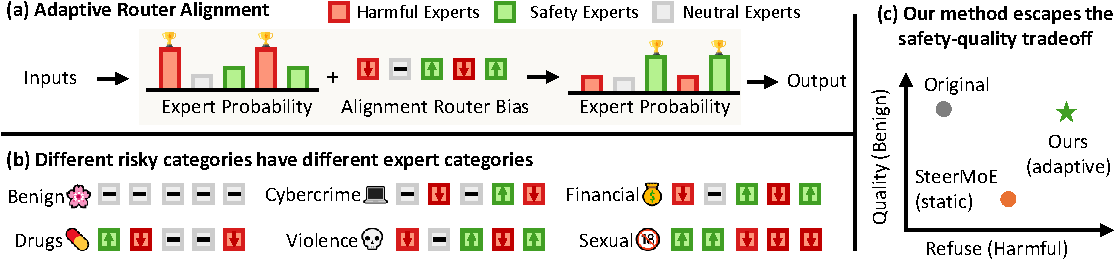
\includegraphics[width=0.88\textwidth,keepaspectratio]{../figures/motivation.pdf}
  \end{center}
  \vspace{-0.4em}
  \footnotesize\centering\itshape\textcolor{mutedgray}{
    We want to (1) skip intervention on benign queries,
    (2) boost only the experts actually about to be used on harmful ones.}
\end{frame}

% ================================================================
% Slide 4: Technique (1) — query-level gate
% ================================================================
\begin{frame}{Technique 1: a query-level ``is this harmful?'' gate \(\lambda(q)\)}
\vspace{-0.5em}
\scriptsize
  \begin{columns}[T]
    \begin{column}{0.54\textwidth}
      \small
      \textbf{Insight.} Intervene \emph{only when}, and \emph{as much
      as}, the query looks harmful and the extent.

      \vspace{0.5em}
      \textbf{How.} Build a linear ``harmful-vs-benign'' direction
      \(\hat d_{\text{refuse}}\) (mean-diff of mid-layer hidden states
      on harmful vs benign prompts, offline), then project each query
      onto it:
      \[
        \lambda(q) \;=\; \mathrm{ReLU}\bigl(h(q)\cdot \hat d_{\text{refuse}}\bigr)
      \]

      \vspace{-0.2em}
      \textbf{Why it works.}
      \scriptsize
      \begin{itemize}\setlength\itemsep{0em}
        \item Benign $\Rightarrow \lambda\!=\!0 \Rightarrow$ defense silent
          $\Rightarrow$ no benign-quality loss.
        \item Risk grows $\Rightarrow \lambda$ grows $\Rightarrow$ defense
          scales naturally --- no hand-tuned threshold.
      \end{itemize}
    \end{column}

    \begin{column}{0.44\textwidth}
      \centering
      \textit{OLMoE-1B-7B-Instruct}\\[0.1em]
      \begin{tabular}{@{}l c c@{}}
        \toprule
        \makecell[l]{~\\}
          & \makecell{Harmful\\refused}
          & \makecell{Benign\\refused} \\
        \midrule
        No defense            & 70\% & 0\% \\
        SteerMoE              & 85\% & \textcolor{harmred}{13.3\%} \\
        \,+\,\textbf{gate}    & \textbf{85\%} & \textcolor{safegreen}{\textbf{0\%}} \\
        \bottomrule
      \end{tabular}\\[0.15em]
      {\tiny\itshape\color{mutedgray} n = 20 harmful + 15 benign prompts,
       judged by Qwen2.5-14B (safe if score $\geq 50$).}
      \vspace{0.4em}

      \textit{Qwen3-Next-80B (under a jailbreak attack)}\\[0.1em]
      \begin{tabular}{@{}l c c@{}}
        \toprule
        \makecell[l]{~\\}
          & \makecell{Harmful\\refused}
          & \makecell{Benign\\score} \\
        \midrule
        Clean (no attack)        & 80\% & 89.3 \\
        Under attack             & \textcolor{harmred}{0\%}  & 89.3 \\
        \,+\,\textbf{gate}       & \textcolor{safegreen}{\textbf{100\%}} & \textcolor{safegreen}{\textbf{91.0}} \\
        \bottomrule
      \end{tabular}\\[0.15em]
      {\tiny\itshape\color{mutedgray} n = 20 harmful prompts under
       jailbreak; benign score on MT-Bench subset.}
    \end{column}
  \end{columns}
\end{frame}

% ================================================================
% Slide 5: Technique (2) — per-expert causal v_e
% ================================================================
\begin{frame}{Technique 2: per-expert harmfulness direction \(v_e\)}
\vspace{-0.2em}
\small
  \textbf{Problem.} SteerMoE uses a \emph{fixed, binary} safe-team
  \(A^{+}\). Too coarse --- ignores which experts are actually useful
  for \emph{this} query.

  \vspace{0.6em}
  \textbf{Idea.} For each expert \(e\), learn a \textbf{harmfulness
  direction} \(v_e\) by asking the model:
  \emph{``which input direction would both raise \(e\)'s routing
  score AND make the final answer a refusal?''}
  \[
    v_e \;=\; \nabla_{h}\bigl[\,\mathrm{gate\_logit}_{e}(h) \;+\;
                               \beta\!\cdot\!\log P(\text{refuse}\mid h)\,\bigr]
  \]

  \vspace{-0.2em}
  \textbf{Per-query, per-expert bias} added to the router gate logit:
  \[
    \text{bias}_e(q,t) \;=\; \alpha\cdot\lambda(q)\cdot
    \langle h(q,t),\, v_e\rangle
  \]
  \vspace{-1.4em}
  \begin{itemize}\setlength\itemsep{0em}
    \item sign \(>0\): expert helps refusal here $\Rightarrow$ \textbf{promote};
    \item sign \(<0\): expert hurts refusal here $\Rightarrow$ \textbf{suppress};
    \item \(\approx 0\): irrelevant expert $\Rightarrow$ left alone.
  \end{itemize}
  One formula, automatically promotes safe experts \emph{and}
  suppresses unsafe ones --- per query, continuously.
\end{frame}

\end{document}
